% ==================================================
% CHAPTER 4: The New Small Wheels %
% ==================================================

\chapter{The New Small Wheels}
\label{chap:nsw}
% Edit count: Lia - 0, Brigitte - 0

% --------------------------------------------------
\section{Motivation for the New Small Wheels}
% --------------------------------------------------

The hit rate of all detector systems will significantly increase during HL-LHC operation because of the increase in luminosity. The increased rate presents a challenge for both the tracking and triggering capabilities of the muon spectrometer~\cite{nsw_tdr}.

In terms of precision tracking, the maximum hit rate in the MDTs is expected to reach above 300 kHz by the end LHC operation.  At this rate, the hit efficiency of MDTs decreases by 35\%, mostly due to the long dead-time of the chambers. Losing hits in the small wheel will reduce the high $p_T$ muon momentum resolution. The decrease in resolution will affect the ability to search for, for example, the decay of hypothetical heavy bosons (W', Z') or other hypothetical particles beyond the SM~\cite{dainese_physics_2018}.

Already during LHC Run-2 operation, the forward muon trigger system had to cope with a very high fake rate, even with the inclusion of TGC data from the small wheel as part of the trigger criteria.  At the luminosity expected in Run-3, it is estimated that 60 kHz out of the maximum L1 trigger bandwidth of 100 kHz would be taken up by forward muon triggers. To address this challenge, a possible solution would be to raise the minimum $p_T$ threshold from \SI{20}{\giga\electronvolt} to \SI{40}{\giga\electronvolt}. However, this would have an adverse impact on the ability to study several physics processes of interest that depend on low $p_T$ muons, particularly the Higgs decay to two muons, the Higgs decay to two tau leptons and hypothetical particle decays beyond the SM~\cite{nsw_tdr}.

The NSWs will address both of these problems. They will be made of precision tracking chambers suitable for the expected hit rates during the HL-LHC and triggering chambers capable of \SI{1}{mrad} track angular resolution. The idea behind the design triggering capability of the chambers is to allow matching of track segments measured by the NSW with track segments from the big wheel to discard tracks not originating from the interaction point. Figure~\ref{fig:nsw_track_triggering} illustrates this point: the Run-2 trigger system would have triggered on all three tracks (A, B, C) while with the NSW the trigger system would only trigger on track A. The NSWs will therefore make it possible to maintain a low muon $p_T$ trigger threshold and maintain an adequate muon momentum resolution during HL-LHC operations, which will allow the full exploitation of the physics potential of this research program~\cite{nsw_tdr}.

\begin{figure}
    \centering
    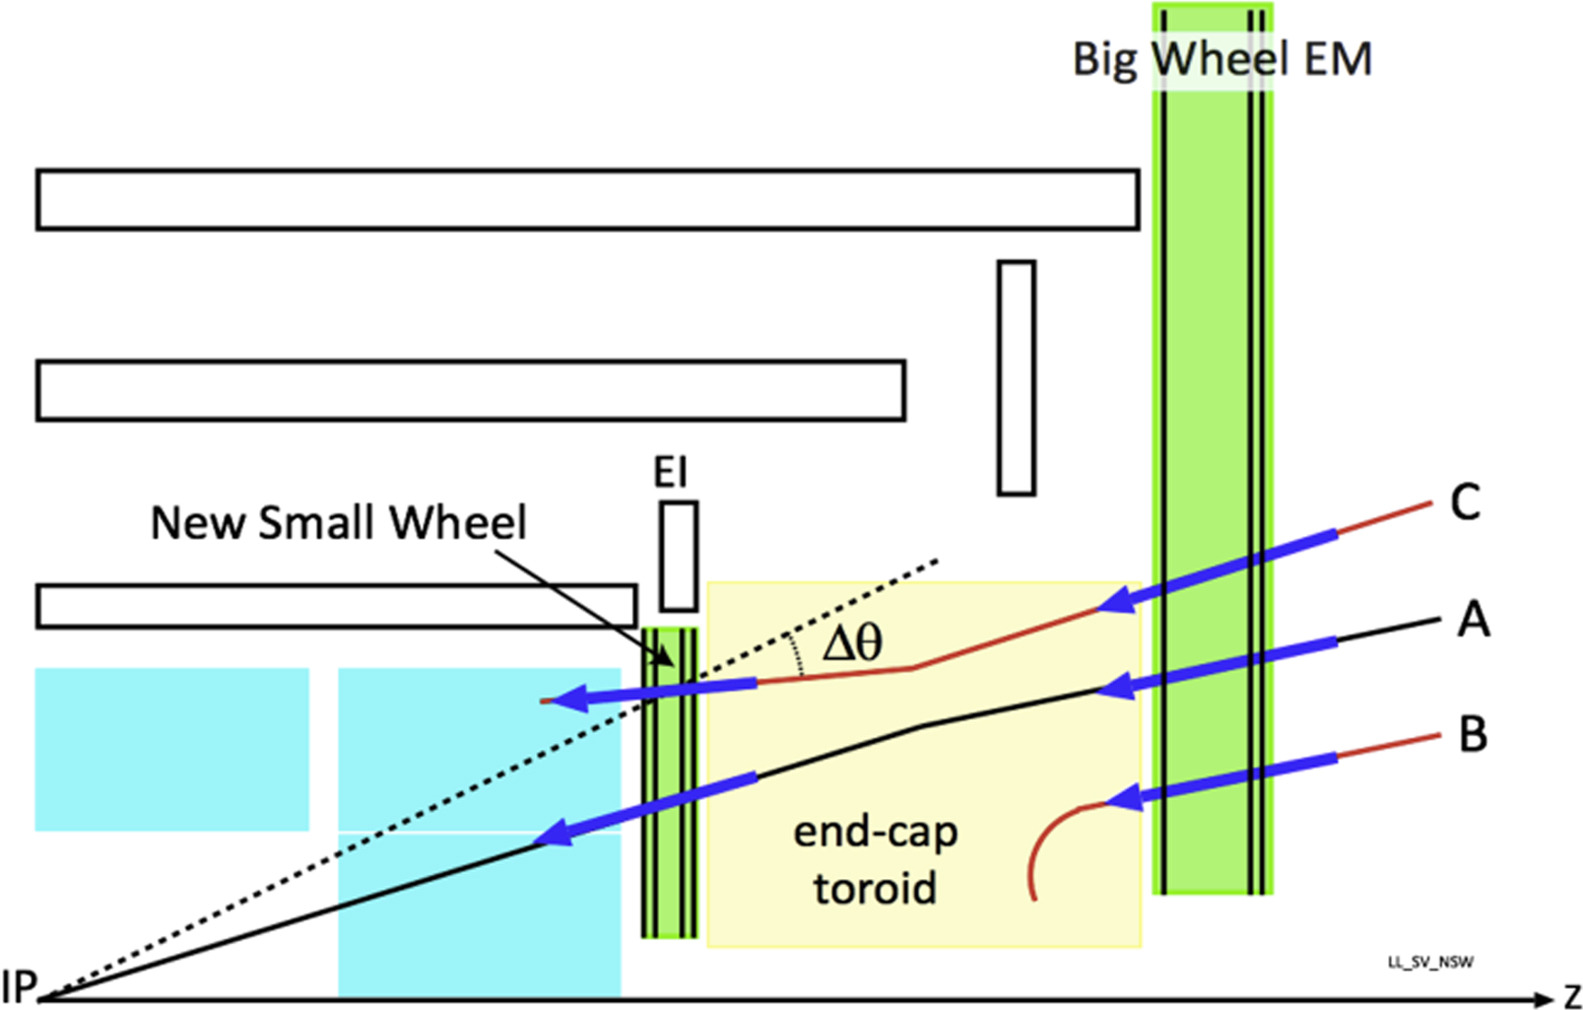
\includegraphics[width = 0.9\textwidth]{figures/perez-codina_NSW_tracks.jpg}
    \caption{A schematic diagram of a quarter cross section of the ATLAS muon spectrometer, with the interaction point (IP) in the bottom left corner. Three possible tracks are labeled. Ideally, track A would be triggered on while track B and C discarded. With the old small wheel, all three tracks would be recorded. With the NSW, only track A would be recorded~\cite{nsw_tdr}.}
    \label{fig:nsw_track_triggering}
\end{figure}

\newpage
\thispagestyle{empty}
\newgeometry{top=0.5in,bottom=0.5in}
\begin{figure}
\centering
\begin{subfigure}{\textwidth}
  \centering
  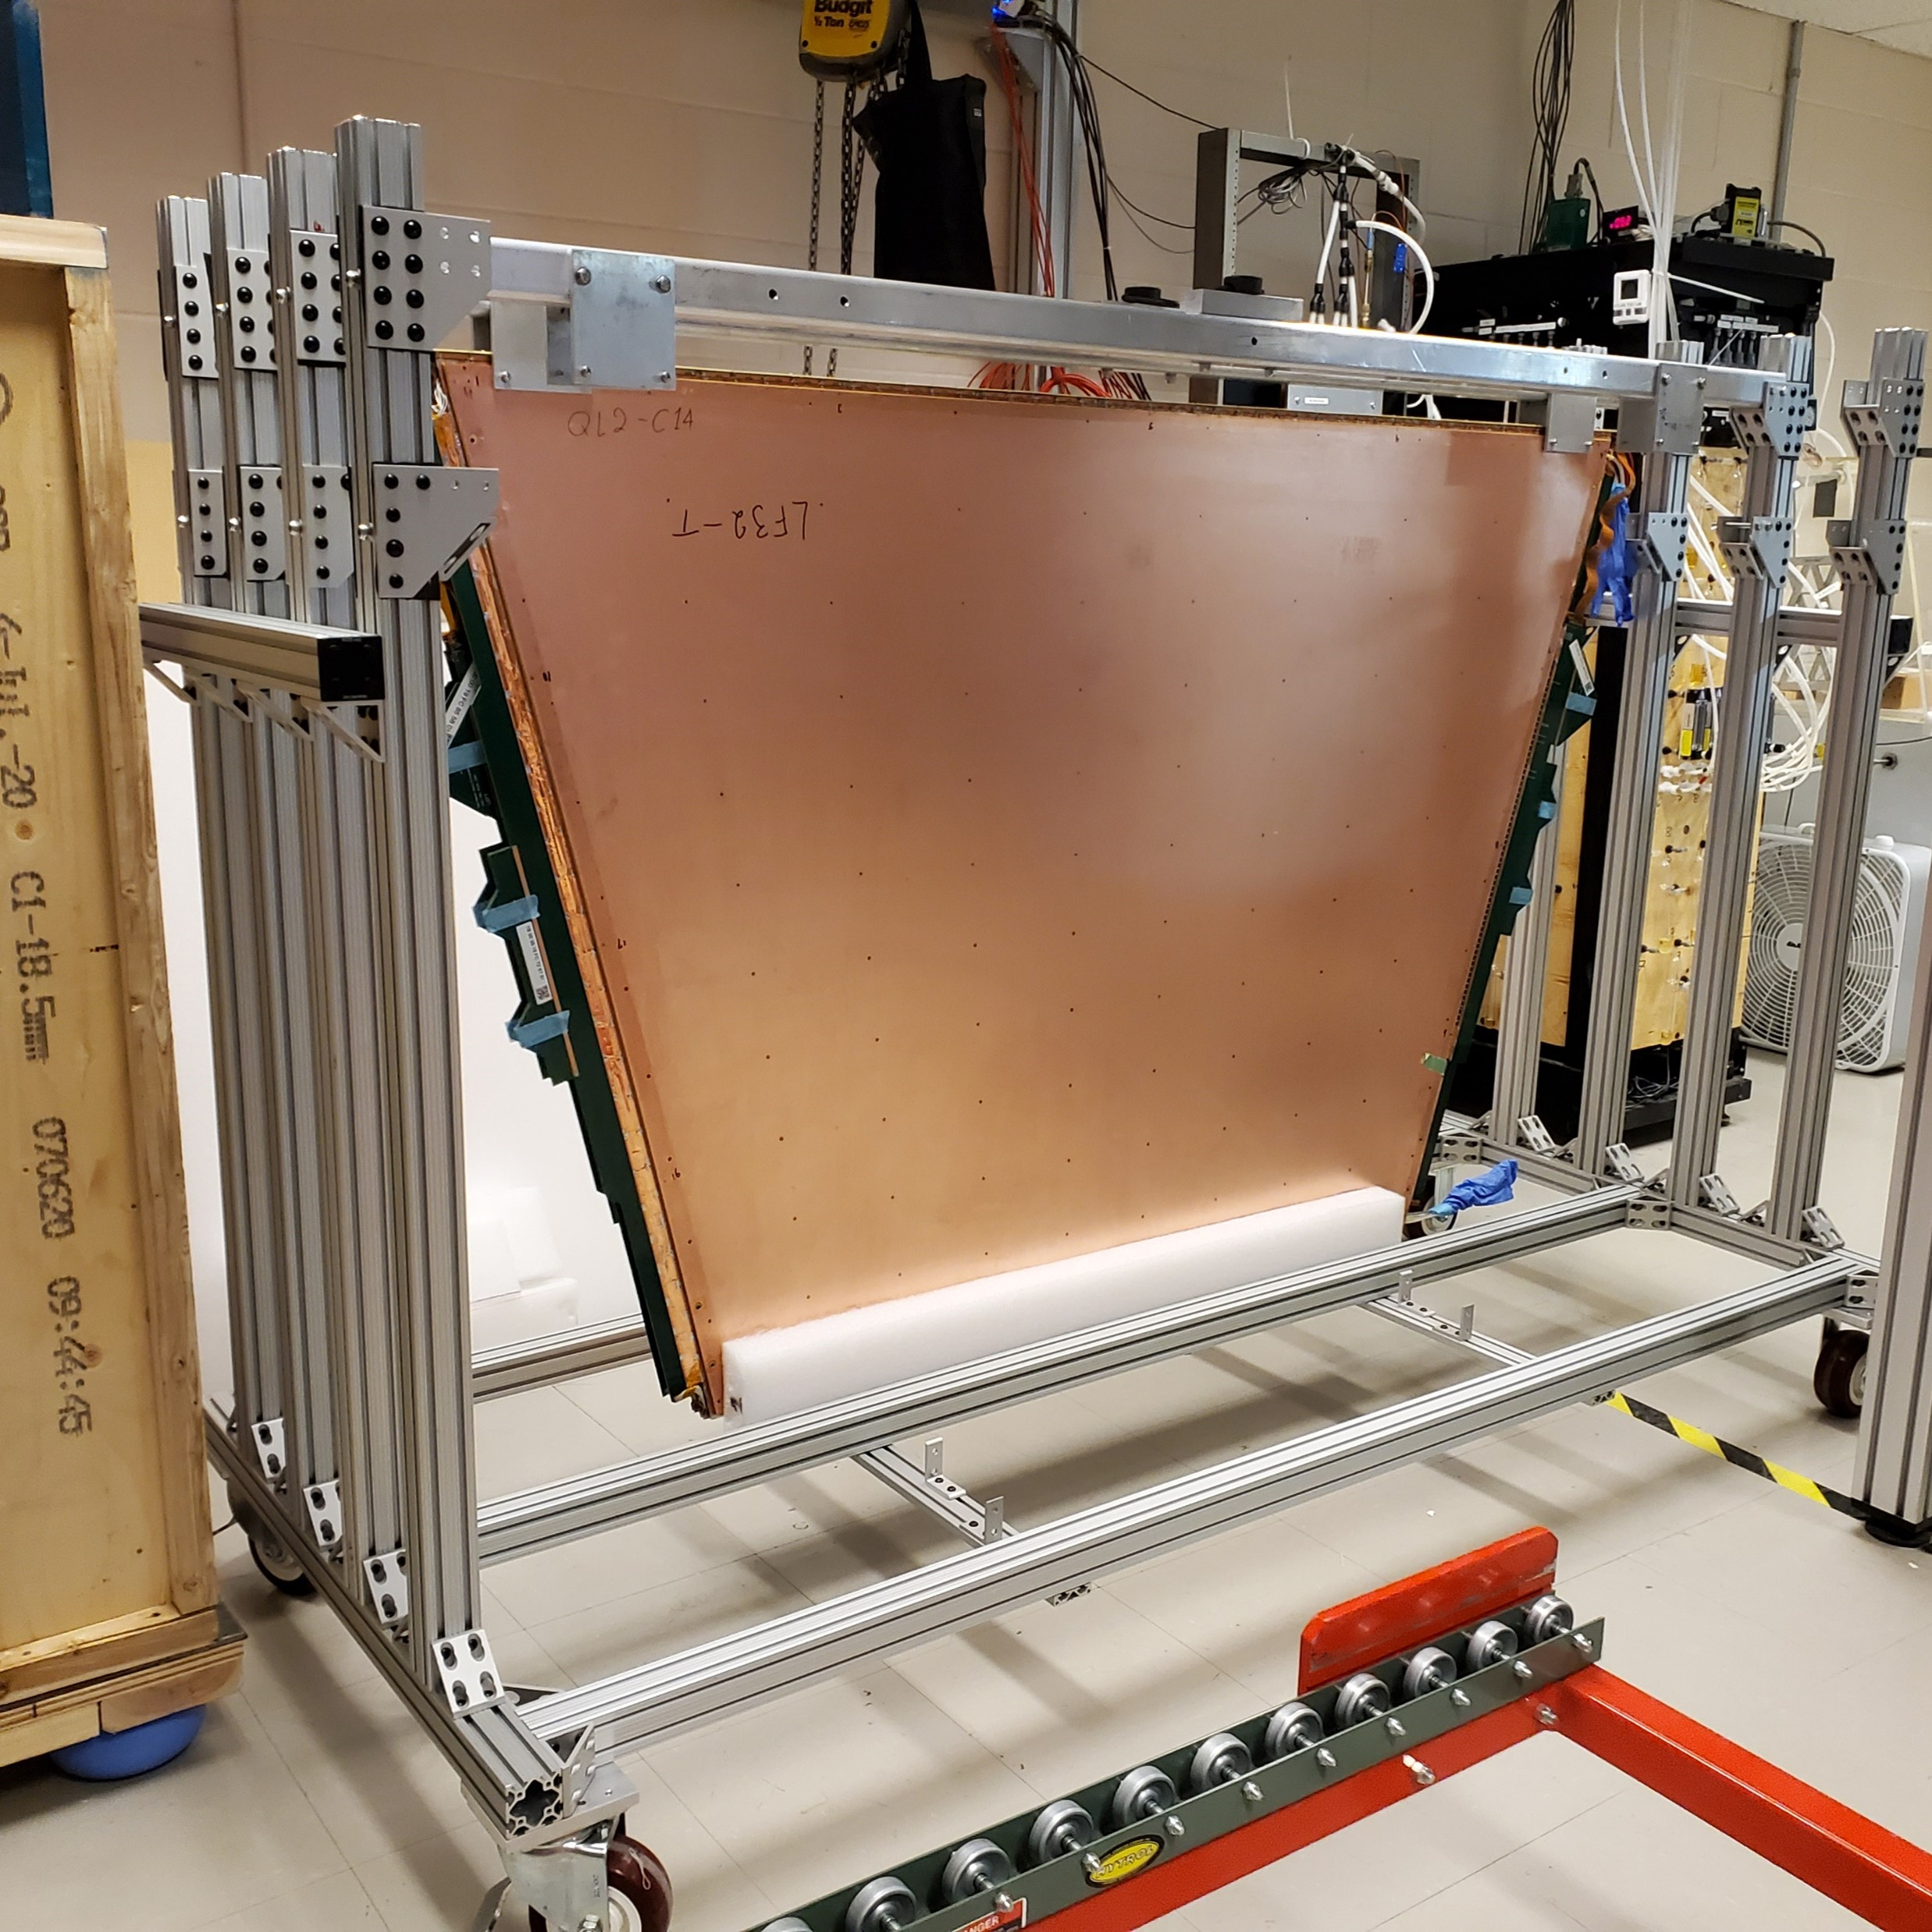
\includegraphics[width=0.35\textwidth]{figures/stgc_quad_cart.jpg}
  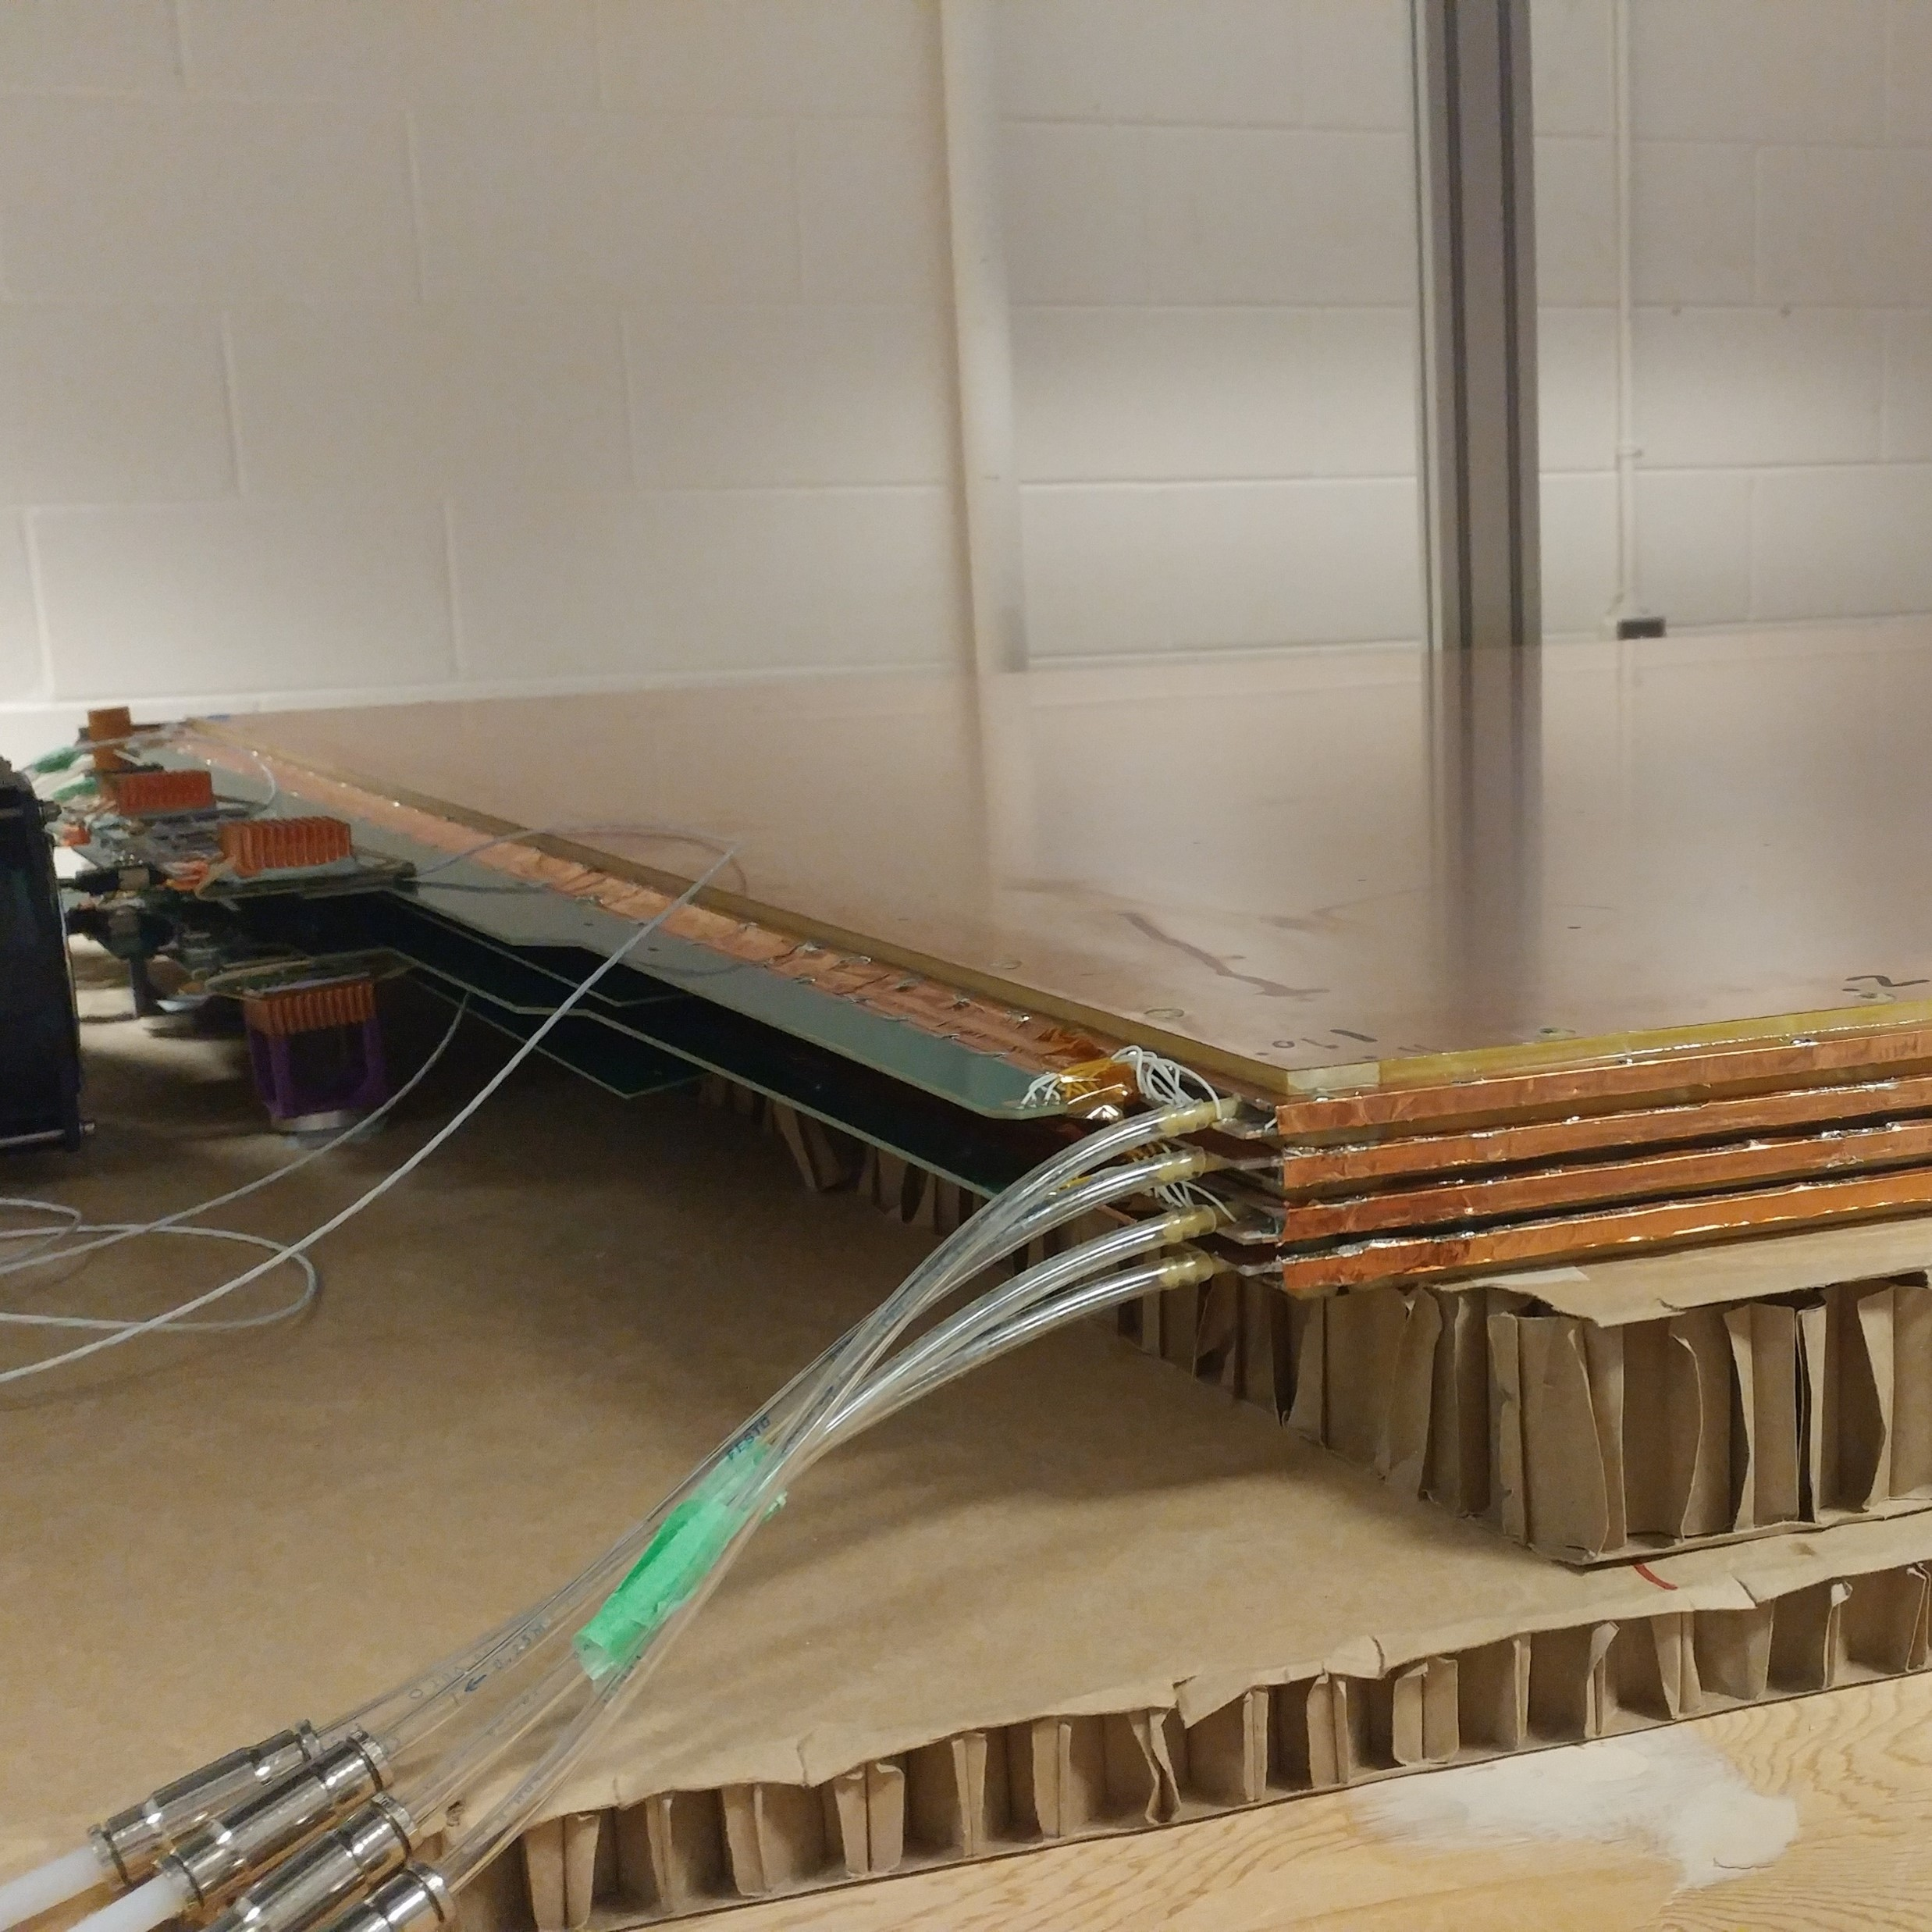
\includegraphics[width=0.35\textwidth]{figures/stgc_quad_inlet_corner.jpg}
  \caption{A sTGC quadruplet module. The left image highlights the trapezoidal shape of a quadruplet module. The right image shows the corner at the short edge, where the four sTGC layers and each layer's gas inlet are visible. The gas outlets and high voltage cables are located along the long edge near the corner in the back left of the photo. The green printed circuit boards along the sides are the adaptor boards where the front end electronics are attached.}
  \label{fig:stgc_quad}
\end{subfigure}

\smallskip

\begin{subfigure}{\textwidth}
  \centering
  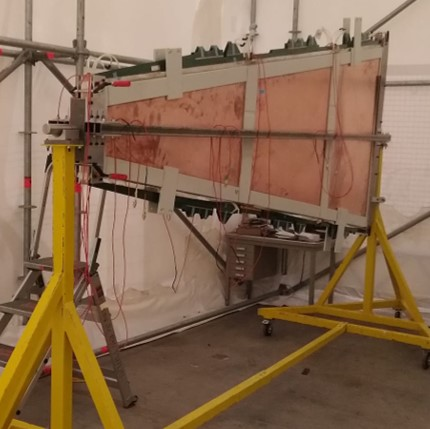
\includegraphics[width=0.35\textwidth]{figures/stgc_wedge.jpg}
  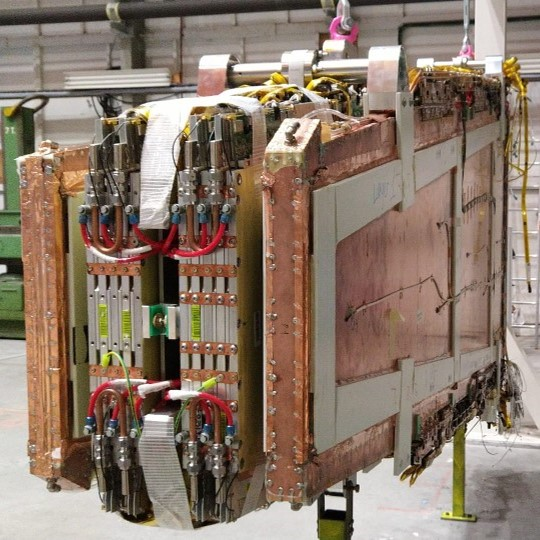
\includegraphics[width=0.35\textwidth]{figures/sector.jpg}
  \caption{Left: A sTGC wedge. The white frame outlines the individual quadruplet modules that have been glued together into a wedge. Right: A completed sector, with two sTGC wedges on the outside and two micromegas wedges on the inside.}
  \label{fig:wedge_and_sector}
\end{subfigure}

\smallskip

\begin{subfigure}{\textwidth}
  \centering
  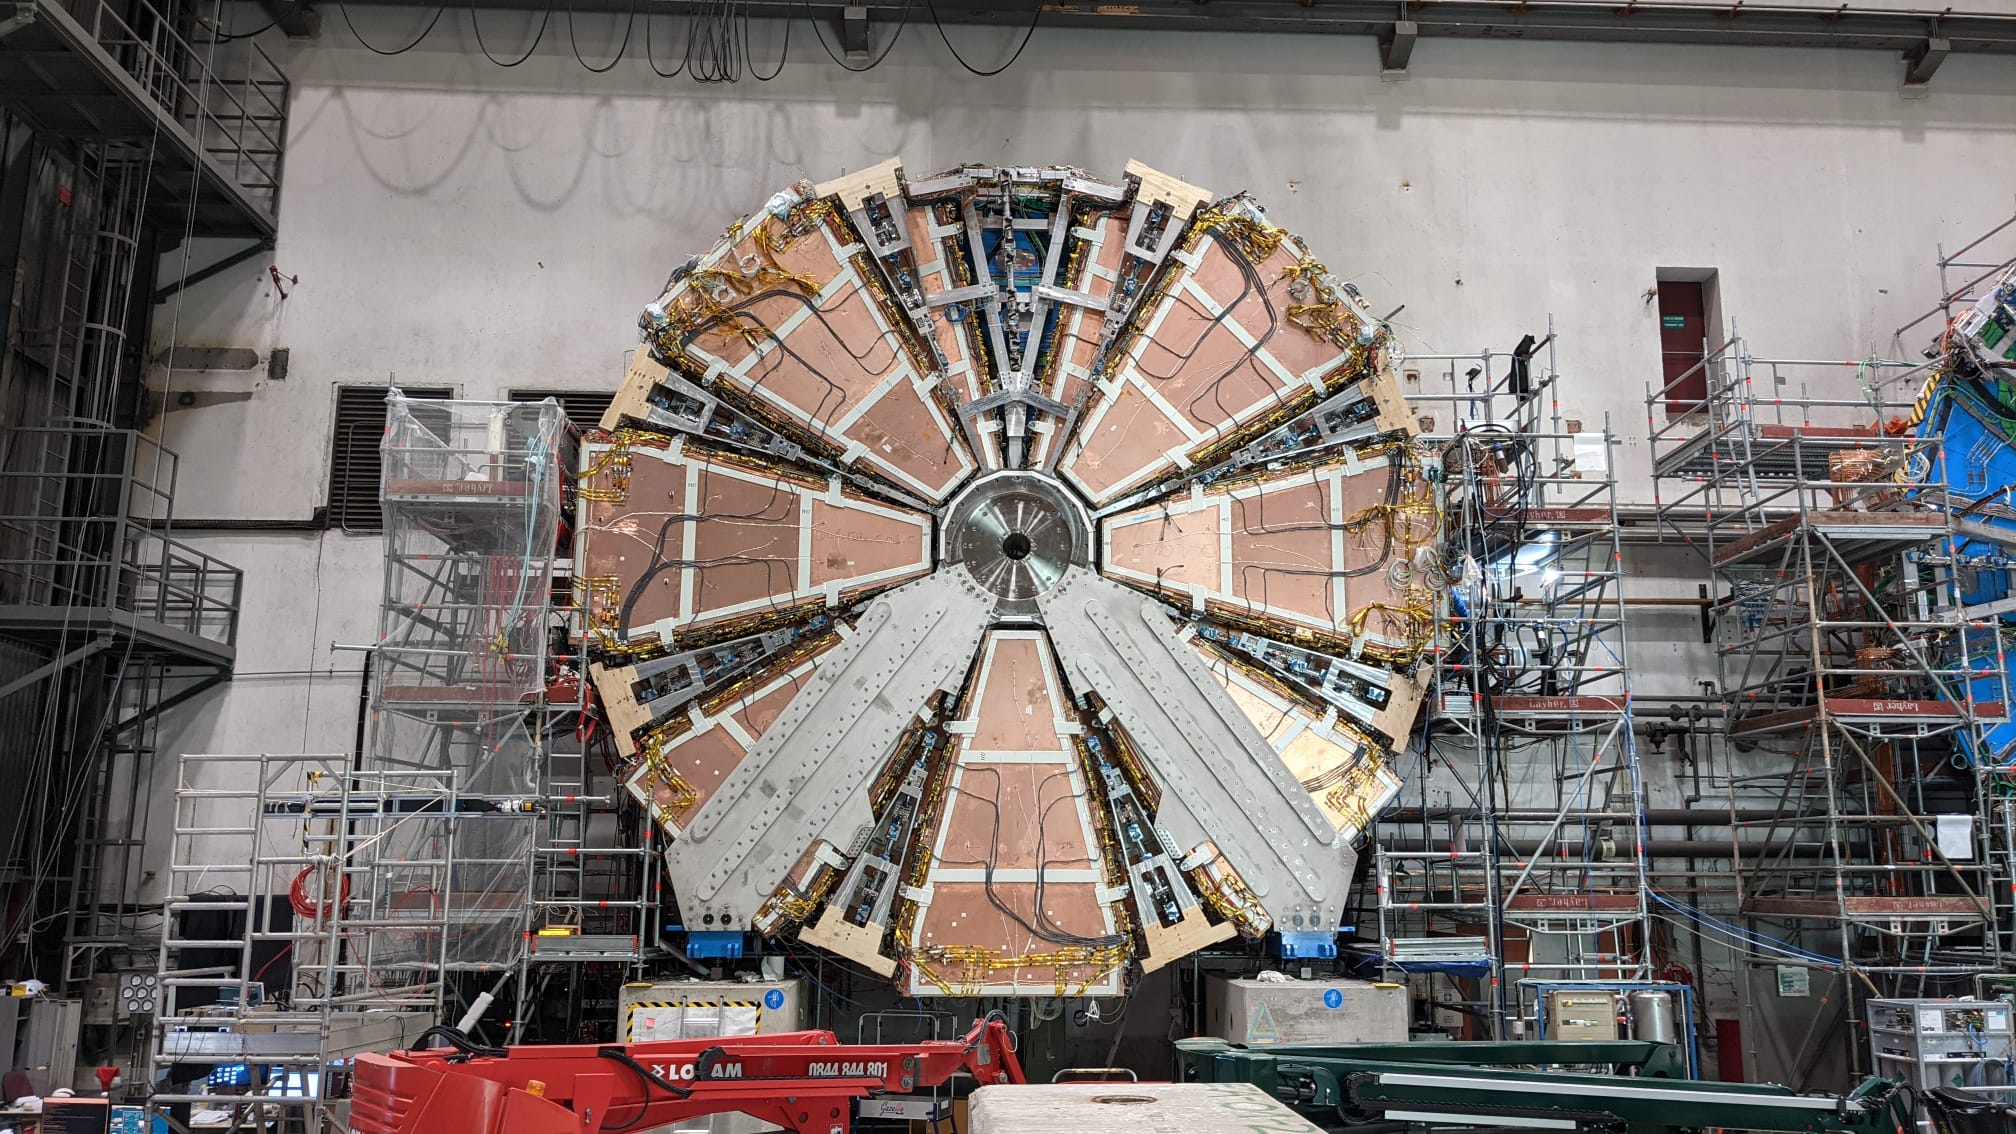
\includegraphics[width=0.7\textwidth]{figures/nsw_2021-05-27_landscape.jpeg}
  \caption{A picture of one of the two NSWs. All sectors except one large sector at the top are installed, revealing two of the smaller sectors that are normally hidden under the large sectors and support bars. The NSWs are \SI{9.3}{m} in diameter. }
  \label{fig:nsw}
  \end{subfigure}
\caption{Images showing different stages of NSW construction.}
\label{fig:nsw_breakdown}
\end{figure}
\newpage
\restoregeometry

% --------------------------------------------------
\section{Design of the NSWs}
% --------------------------------------------------

The NSWs are made with two detector technologies: micromegas and small-strip thin gap chambers. Eight layers of each cover the entire area of the wheel. Micromegas are designed to be the primary precision tracking detectors and sTGCs the primary triggering detectors, but both technologies offer full redundancy by being capable of providing both precision measurements and trigger information. Both types of detectors were designed to achieve spatial resolution better than $\sim$\SI{100}{\micro\meter} per layer. Four chambers are glued together to create quadruplet modules of each detector type. Quadruplets of different sizes, most shaped as trapezoids, are assembled into wedges. Two sTGC wedges and two micromegas wedges are layered to create sectors (with the sTGC wedges on the outside)~\cite{nsw_tdr}. Different stages of the construction process are shown in Figure~\ref{fig:nsw_breakdown}. At the time of writing, the assembly of the NSWs has just been completed. The first NSW has been lowered into the ATLAS cavern and is being commissioned and the second will be lowered shortly. 

% \textcolor{red}{\textit{for if you use computer generated NSW diagram}} Sectors covered the wheel, as shown in figure~\ref{fig:nsw_diagram}. Practically, two different wedge sizes, small and large, were required to completely cover the wheel.
% \begin{figure}
%    \centering
%    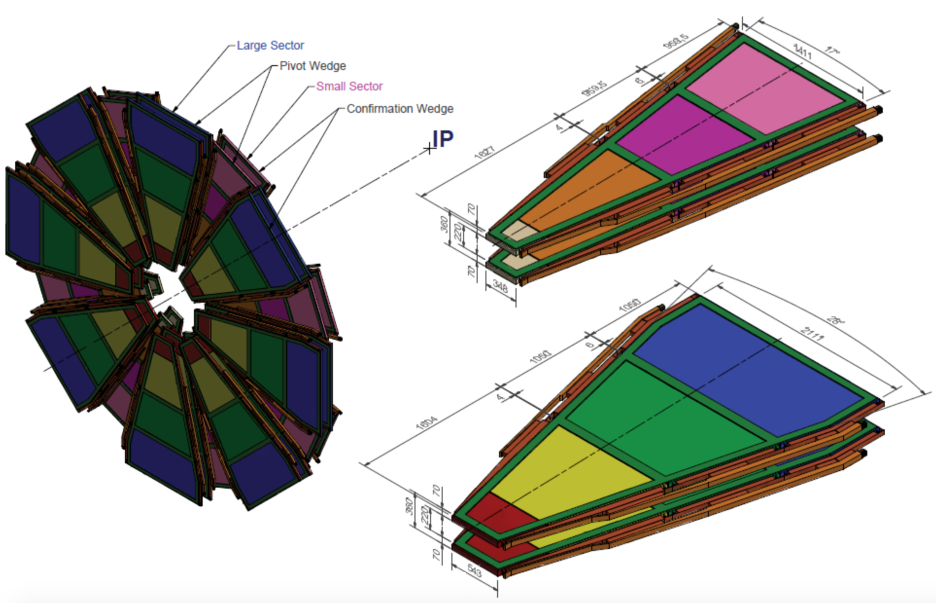
\includegraphics[width = 0.9\textwidth]{figures/nsw_diagram.png}
%    \caption{Drawing of the new small wheel, and diagrams of the individual small and large wedges. Each colour represents a different sTGC module size.}
%    \label{fig:nsw_diagram}
% \end{figure}
% ORIGINAL FULL PAGE NSW SPREAD POSITION

% --------------------------------------------------
% \section{Micromegas}
% --------------------------------------------------

% Micromegas have three components: a drift plane, a gas gap, a mesh, and readout strips, as shown in figure~\ref{fig:micromega}. High voltage is applied to the readout strips. An ionization event in the gas causes electrons to drift towards the mesh. Once they arrived, they are amplified by the strong field and the avalanche is picked up by the readout electrodes. The small distance between the readout electrodes and the mesh, \SI{128}{\micro\meter}, means that positive ions are evacuated in $\sim$\SI{100}{\nano\second}, making micromegas a good choice for high rate environments~\cite{nsw_tdr}. The small pitch of the readout electrodes, \SI{0.425}{mm}, provides spatial resolution much better than \SI{100}{\micro\meter}~\cite{stelzer_new_2016}. MM quadruplets will be used for offline precision tracking~\cite{nsw_tdr}.

% \begin{figure}
%    \centering
%    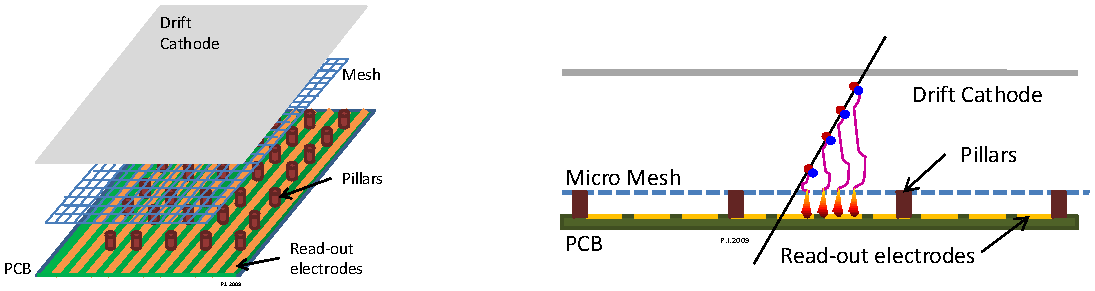
\includegraphics[width = 0.9\textwidth]{figures/micromegas.png}
%    \caption{Sketch the micromega operating principle. Positive high voltage is applied to the readout electrodes, which creates a strong field between the mesh and the readout electrodes, and a weaker field between the mesh and the drift cathode. Amplification takes place between the readout electrodes and the mesh. Figure from~\cite{nsw_tdr}}
%    \label{fig:micromega}
% \end{figure}

% --------------------------------------------------
\section{Small-strip thin gap chambers}
% --------------------------------------------------

\begin{figure}[t]
    \centering
    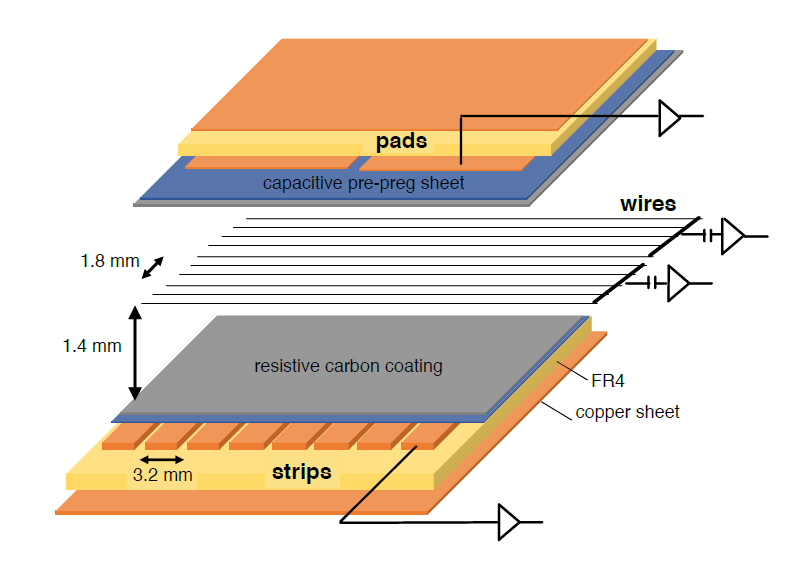
\includegraphics[width = 0.9\textwidth]{figures/stgc_internals.png}
    \caption{Interal structure of an sTGC, zoomed into the area under a pad. High voltage is applied to wires suspended in the gas volume to create an electric field. A passing muon causes an ionization avalache that is picked up by the wire, strip and pad electrodes~\cite{lefebvre_precision_2020}.}
    \label{fig:stgc_internals}
\end{figure}

The sTGCs are gas ionization chambers operated with a gas mixture of CO$_2$:n-pentane with a ratio of 55\%:45\% by volume. Gold-plated tungsten anode wires, \SI{50}{\micro\meter} in diameter and with \SI{1.8}{mm} pitch, are suspended between two cathode planes made of FR-4 printed circuit board, each \SI{1.4}{mm} away (see Figure~\ref{fig:stgc_internals}). One cathode board is segmented into copper pads of varying area (with a typical size of $\sim$\SI{300}{cm^2} each), and the other is segmented into copper strips of \SI{3.2}{mm} pitch running lengthwise perpendicular to the wires. High voltage is applied to the anode wires and the cathode planes are grounded~\cite{nsw_tdr, perez-codina_small-strip_2016}. When a muon passes through a sTGC, it will ionize nearby atoms of the gas. The electrons drift towards the anode wires and in the high electric field region near the wires generate an ionization avalanche~\cite{townsend_electricity_1915}. The motion of the ions and free electrons generates small currents on the nearby wire and capacitatively-coupled strip and pad electrodes~\cite{nsw_tdr}. The gas mixture was chosen to absorb excess photons produced in the avalanche that delocalize the avalanche signal~\cite{majewski_thin_1983} and saturate many strip electrodes, preventing the formation of streamers~\cite{grupen_particle_2008}.  This allows the chambers to be run at a higher high-voltage providing a faster response and higher signal~\cite{majewski_thin_1983}. A carbon coating and pre-impregnated sheet are layered over the printed circuit board of the cathode board, as shown in Figure~\ref{fig:stgc_internals}. The resitivity of the carbon coating and capacitance of the pre-impregnated sheet tune the spread of the charge distribution~\cite{gatti_optimum_1979} and the speed of the response~\cite{battistoni_resistive_1982} to optimize the rate capability. The combined information from the strip readout electrodes and wires provide the location where the muon passed through the chamber. The small pitch of the strip readout electrodes is what allows the quadruplets to deliver good track angular resolution to improve the fake trigger rate and meet the precision tracking requirements~\cite{nsw_tdr}.

% comment on "quick enough to be provided as input to the L1 trigger. Pg. 131 of NSW TDR states req' is under 1025 ns for phase-1, phase-2 will allow longer latency. Latency predictions are shown on pg. 146, but are mostly estimates. Not sure where these latencies are actually measured, nor what the phase-2 requirement is.
A 3-out-of-4 coincidence in pad electrodes from each layer of a quadruplet defines a region of interest where the strip and wire electrodes should be read out. The pad triggering scheme greatly reduces the number of electrodes that require readout so that a track segment of the required angular resolution can be provided quickly enough to the hardware trigger~\cite{nsw_tdr}.

Signal is read out from groups of 20 successive wires, so the position resolution in the direction perpendicular to the wires is \SI{10}{mm} per plane. The wires give the azimuthal coordinate in ATLAS so the position resolution in this direction is sufficient. Good resolution on the $\eta$ coordinate, perpendicular to the strips, is important~\cite{nsw_tdr}. In a test beam environment, the strip spatial resolution of a single sTGC was measured to be 45 microns for muons perpendicularly incident on the surface of the sTGC.  Although the spatial resolution worsens as function of muon angle measured from normal incidence~\cite{lefebvre_thesis}, when four sTGCs are glued together into a quadruplet the design angular resolution of \SI{1}{mrad} in the strip coordinate is achievable~\cite{nsw_tdr, perez-codina_small-strip_2016}. 

To achieve the required track angular resolution once installed in ATLAS, the absolute position of each sTGC strip within the ATLAS coordinate system must be accurately known. The degree of accuracy required is on the order of the position resolution of the chambers, $\sim$\SI{100}{\micro\meter}. The NSW alignment system, detailed in Section~\ref{sec:nsw_alignment}, will monitor the position of alignment platforms installed on the surface of the wedges. The alignment platforms are installed with respect to an external reference on the sTGCs: two brass inserts on each strip layer on one of the angled sides of each quadruplet (shown in Figure~\ref{fig:brasses}). So the challenge of monitoring the position of the strips in ATLAS was separated into two steps: first, infer the position of the strips with respect to the brass inserts using the sTGC design geometry; second, use the alignment system to monitor the position of the alignment platforms. The next section provides some pertinent details on the sTGC construction process, with steps that affect the position of the strips with respect to the brass inserts highlighted.
% The position of the strips can be separated into two stages. First, the NSW alignment system monitors the position of alignment platforms installed on the surface of the wedges, as detailed in section~\ref{nsw_alignment}. Second, the internal geometry of the chambers must be referenced with respect to the wedges. Parts of the sTGC construction process that affect the position of the strips are explained in section~\ref{sec:stgc_construction}. The chapter closes 

\begin{figure}
\centering
\begin{subfigure}{.5\textwidth}
  \centering
  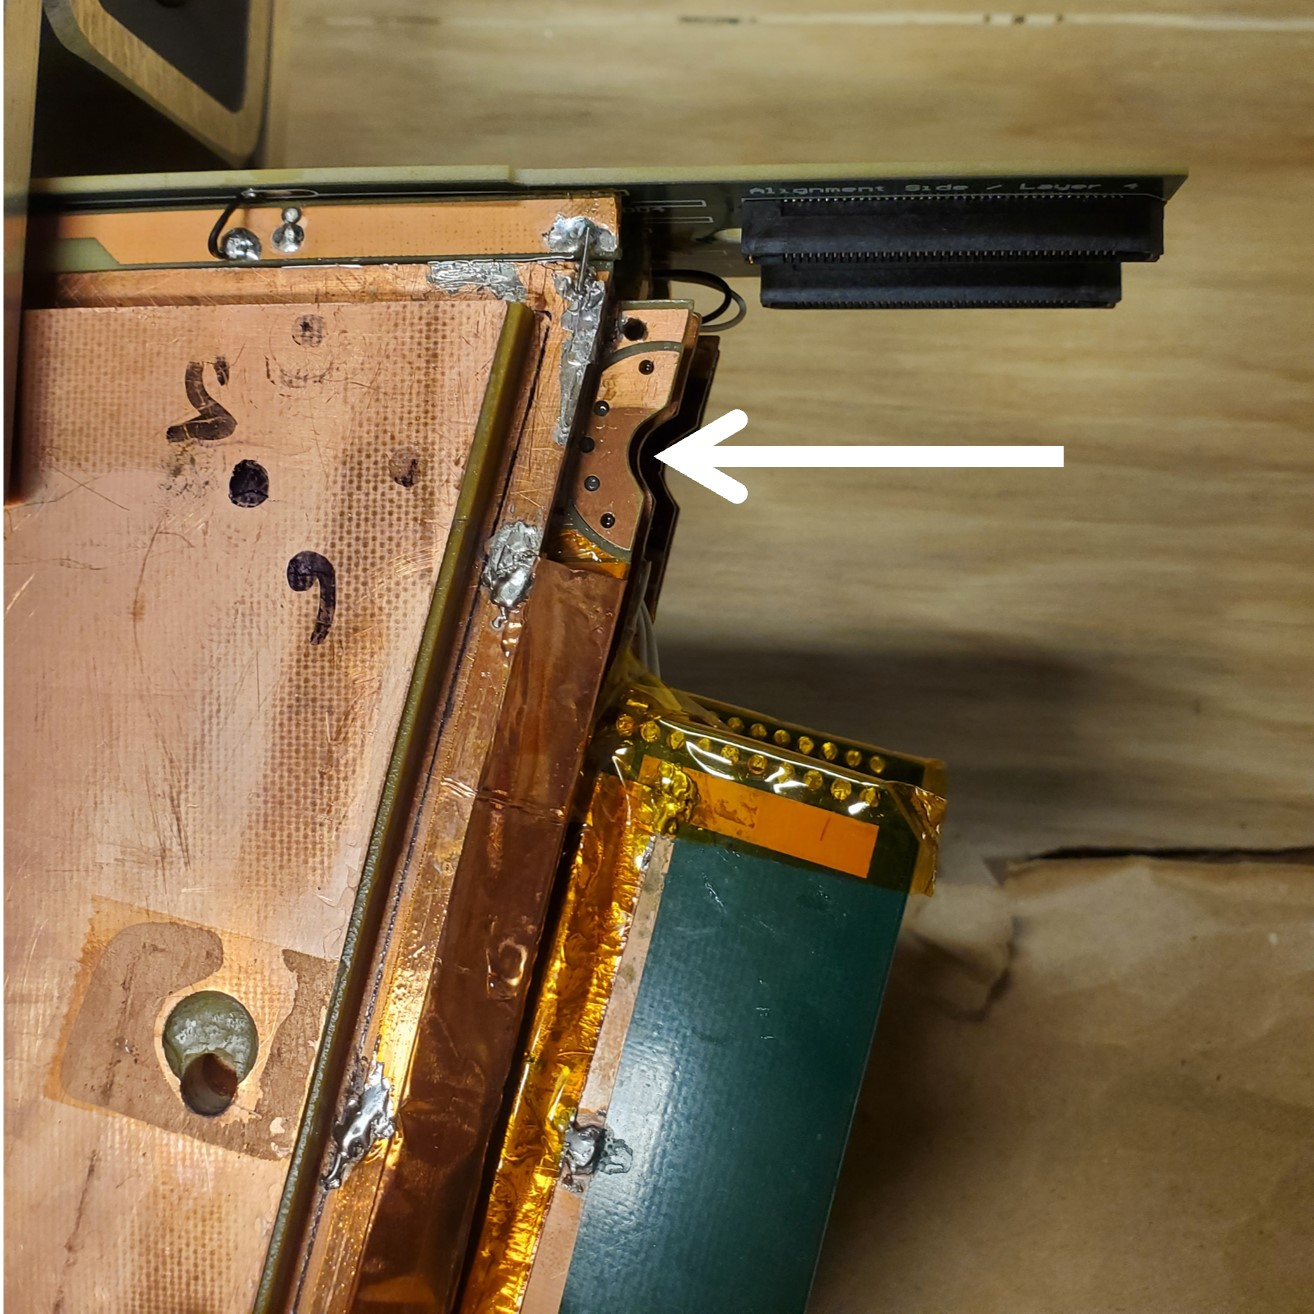
\includegraphics[width=\linewidth]{figures/brass_top.jpg}
  \caption{Brass insert near long edge.}
  \label{fig:brass_top}
\end{subfigure}%
\begin{subfigure}{.5\textwidth}
  \centering
  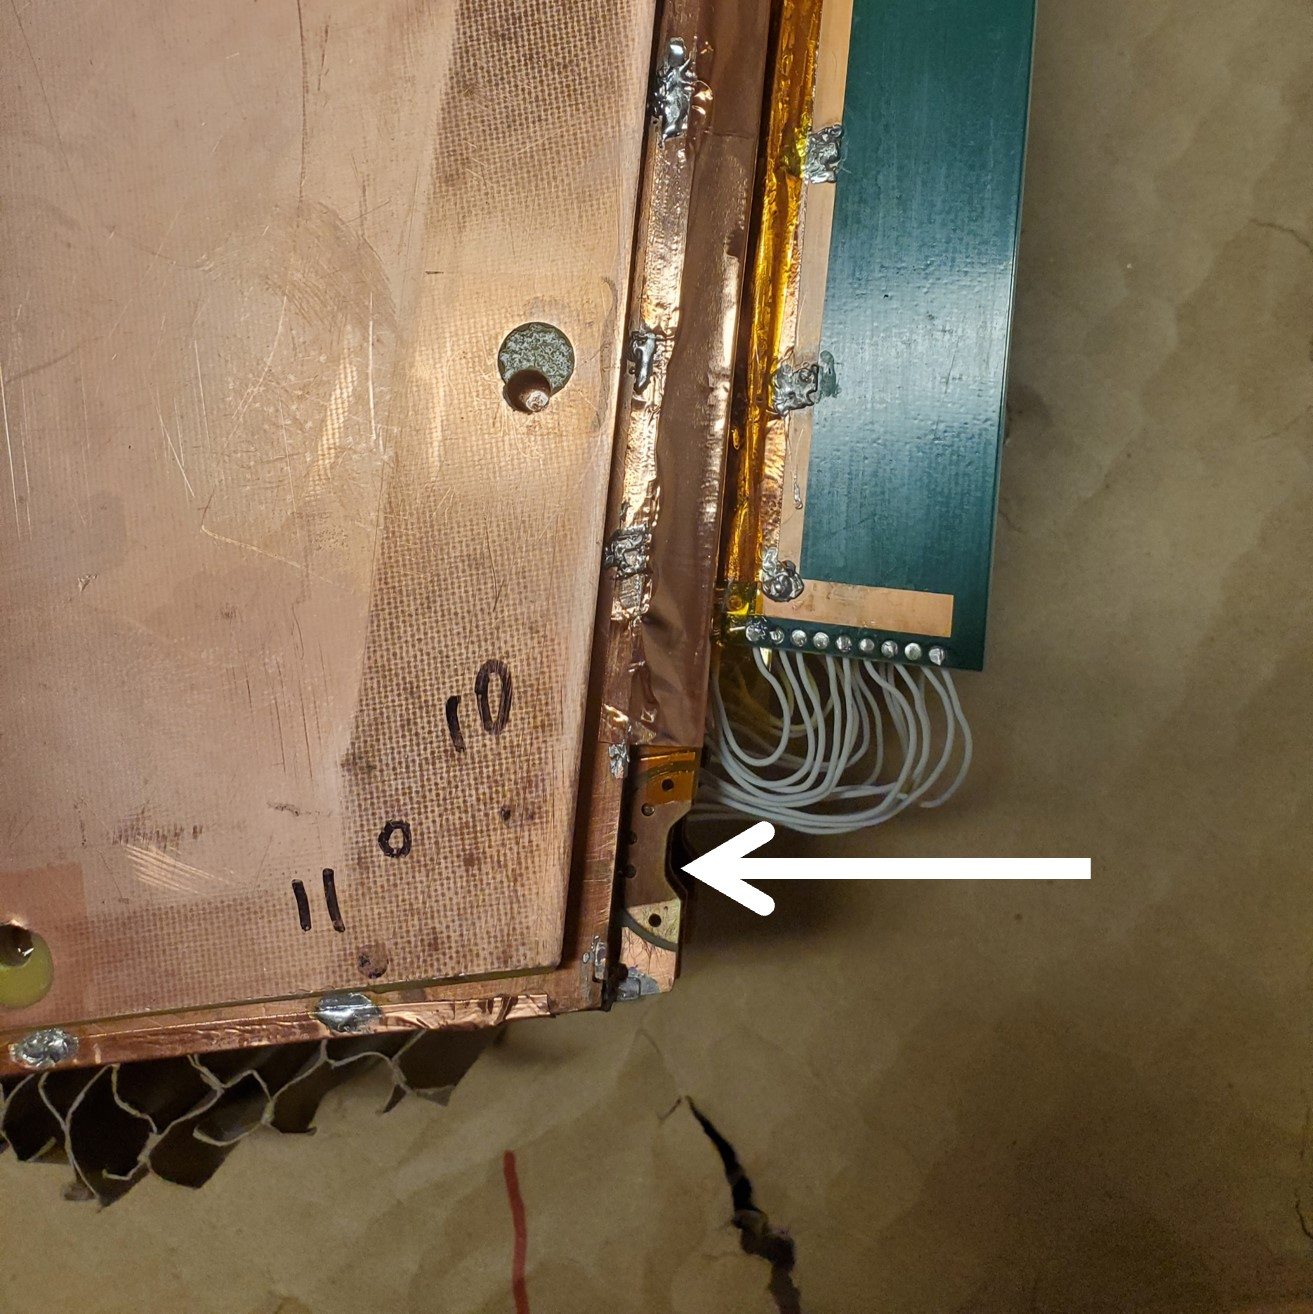
\includegraphics[width=\linewidth]{figures/brass_bottom.jpg}
  \caption{Brass insert near short edge.}
  \label{fig:brass_bottom}
\end{subfigure}
\caption{The brass inserts sticking out from the gas volumes of an sTGC quadruplet. These inserts were pressed against alignment pins when the individual sTGCs were being glued together.}
\label{fig:brasses}
\end{figure}

% However, the accuracy of the hit positions on each layer depends on how well the position of the strips are known in the ATLAS coordinate system. 

% Each strip cathode board has two brass inserts, one near the long edge and one near the short edge, pictured in Figure~\ref{fig:brasses}. The inserts were used to align the strip layers of a quadruplet during construction. They were supposed to control the position of the strips to within \SI{40}{\micro\meter} within nominal. The idea was that the NSW alignment system would monitor the position of points on the surface of an sTGC wedge (discussed in section~\ref{sec:nsw_alignment}) and that the combined external and internal alignment uncertainty on the strip positions would be acceptably small for the precision tracking goals~\cite{nsw_tdr}. Uncontrolled offsets of strip positions on an sTGC layer will bias the reconstructed hit position and hence the track, reducing accuracy of the momentum measurement. To understand the source of offsets in strip positions and misalignments between strip layers, pertinent details of the sTGC construction process are presented in the next section.

% In addition, the sTGC quadruplets should be able to provide precision tracking within \SI{100}{\micro\meter} per plane in the event of a MM module failure.

% --------------------------------------------------
\section{sTGC Quadruplet Construction}
% --------------------------------------------------
\label{sec:stgc_construction}

Five countries were responsible for producing sTGC quadruplets of varying geometries for the NSW: Canada, Chile, China, Israel and Russia. Canada was responsible for the construction of one quarter of the required sTGCs, of three different quadruplet geometries. The steps of the construction process in each country were similar~\cite{nsw_tdr}. The process followed in Canada is detailed here.

A research group at TRIUMF in Vancouver, British Columbia was responsible for preparing the cathode boards. The boards were made and the electrodes etched on at a commercial laboratory, Triangle Labs, in Carson City, Nevada. Once completed they were sent to TRIUMF to be sprayed with graphite and to have support structures glued on~\cite{carlson_results_2019}. The boards are commercial multilayer printed circuit boards, but the strip boards required precision machining to etch the strip pattern~\cite{nsw_tdr}. Triangle Labs also machined the two brass inserts into each strip board. A coordinate measuring machine (CMM) was used to accurately measure the position of a set of reference strips on each board. Four quality parameters describing non-conformities in the strip pattern of each board with respect to the brass inserts were derived from the data and the results are available on a QA/QC database. The parameters~-- offset, angle, scale and nonparallelism~-- and the CMM data collection is described in full in~\cite{carlson_results_2019}.  Due to time constraints, tolerances on the non-conformities in the etched strip pattern with respect to the brass inserts were loosened, with the condition that the strip positions in ATLAS would have to be corrected for~\cite{carlson_results_2019}. 

The prepared boards were sent to Carleton University in Ottawa, Ontario for construction into sTGCs and quadruplets. First, the wires were wound around the pad cathode boards using a rotating table and the wires were soldered into place. A wound pad cathode board was held by vacuum on a granite table, flat to within \SI{20}{\micro\meter}, and a strip cathode board glued on top to create an sTGC. Holding one sTGC flat with the vacuum, another was glued on top to create a doublet, then two doublets were glued together to create a quadruplet. When gluing sTGCs together, the brass inserts were pushed against alignment pins with the goal of keeping the strip layers aligned within tolerance. However, non-conformities in the shape of the brass inserts, non-conformities in the position of the alignment pins and shifts between sTGCs while the glue cured resulted in misalignments between the brass inserts and strip layers. Precise alignment of the pad boards or wires with respect to the strip boards did not have to be so tightly controlled because pads and wires do not measure the precision coordinate. 

The Carleton team finished the quadruplets by installing adaptor boards on the angled sides of each layer that allow front end electronics to be attached. Completed quadruplets were sent to McGill University where their performance was characterized with cosmic rays. Details pertaining to cosmic ray testing of sTGC quadruplets at McGill University are described in Chapter~\ref{chap:cosmics}. Tested quadruplets were sent to CERN where they were assembled into wedges and alignment platforms installed. The alignment platforms were installed using a jig positioned with respect to the brass inserts. Completed wedges were assembled into sectors then installed on the NSWs.

% So, during cathode board construction the etched strip pattern could be shifted off of nominal with respect to the brass inserts. While gluing sTGCs together, non-conformities in the shapes of the brasses and the position of the alignment pins resulted in misalignments between the brass inserts that mean they are not a uniform reference for every layer of the quadruplet. 

The quadruplet construction process had two steps where strip positions could be shifted off nominal. At board-level, there could be non-conformities in the etched strip pattern with respect to the brass inserts, described by the four quality parameters~\cite{carlson_results_2019}. At the quadruplet level, misalignments between the brass inserts and strips on different layers were possibly introduced during the gluing. The result was that the brass inserts were not a reliable reference point and that the strips can be offset from their design position by up to hundreds of micrometers. Offsets in strip positions from nominal in Canadian quadruplets were shown to be random~\cite{carlson_results_2019}, so no one correction would suffice. The offsets must be measured and corrected for in the ATLAS offline software that does the precision tracking. Understanding the work ongoing to make measurements of strip position offsets and correct for them requires understanding the strategy of the NSW alignment system.

% Two sources of misalignment resulted at board level: non-conformities in the placement and shape of the brass inserts and non-conformities in the strip pattern. Carlson addressed the non-conformities in the strip pattern of Canadian cathode boards in his thesis~\cite{carlson_results_2019}. A coordinate measuring machine (CMM) or FaroArm was used to digitize the etched strip pattern of each board. Four quality parameters describing non-conformities in the strip pattern were derived from the data and the results are available on a QA/QC database. The parameters were offset, angle (rotation), scale and non-parallelism, defined in ful in Carlson' thesis. Often, alignment models only consider an offset and rotation. 

% Once the cathode boards were prepared, they were sent to TRIUMF in Vancouver, British Columbia to be sprayed with the graphite coating. After spraying, the coating was polished until the resistivity was between 90 and \SI{110}{\kilo\ohm}$/\msquare$, then wire support structures and frames were installed~\cite{nsw_tdr}. The completed boards were sent to Carleton university for construction into gas gaps and multiplets.

% First, anode wires were wound onto the the pad cathode boards using a rotating vacuum table. Then, a pad and strip cathode board has to be glued together to create an sTGC, two sTGCs glued together to create a doublet, and two doublets glued together to create a quadruplet. Gluing was done by holding one side of a cathode board in place with vacuum on a granite table, flat to within \SI{20}{\micro\meter}. A honey comb spacer separates each sTGC layer of a quadruplet. When closing a gas gap, micrometer misalignments between the strip and pad cathode boards do not matter since the pads do not measure precision coordinates. When gluing sTGCs into doublets however, alignment between strip layers had to be controlled by pushing the two brass inserts against alignment pins~--- similarly for gluing together doublets. Once a quadruplet was assembled, adapator boards used to route the electrodes' signals to the front end electronics were soldered on to the angled sides of the quadruplet~\cite{nsw_tdr}. 

% If you want to include the x-ray survery of the brass positions and the microscope method
% At every stage in the process quality control checks were in place for gas, high voltage, and alignment. For alignment, \textcolor{red}{the position of the brasses were recorded in 3D using an x-ray gun~\cite{nsw_tdr} \textit{--> Did this actually happen?}}~\cite{nsw_tdr} and alignment between strips visible outside a quadruplet was checked with a microscope~\cite{carlson_results_2019}. 

% Quality control tests of alignment, ability to hold high voltage, gas sealing etc. were undertaken at every stage in the construction process~-- details can be found in~\cite{nsw_tdr}. The final set of quality control checks and characterization was done at McGill University in Montreal, Quebec. Completed quadruplets were tested for gas leaks, noise and characterized with cosmic rays. The details of cosmic ray testing are described in chapter~\ref{chap:cosmics}.

% Once the quadruplets have been tested with cosmics rays, they are sent to CERN to be further tested, assembled into wedges then sectors, then installed on the NSWs. At the time of writing, all sectors have been installed on both wheels. The first NSW has been lowered into the ATLAS cavern and is being commissioned. The second is scheduled for installation in October, 2021.

% --------------------------------------------------
\section{NSW alignment}
% --------------------------------------------------
\label{sec:nsw_alignment}
% The idea of the NSW alignment system is presented in~\cite{nsw_tdr}, but the details have only been presented internally so far. The original goal of the alignment system was to provide the position with respect to one another of any three chambers traversable by a muon track with an accuracy of \SI{40}{\micro\meter} in the precision coordinate~\cite{nsw_tdr}. Likely for sTGCs, this will mean inputing the strip postions, or parameters to calculate the strip positions, into the ATLAS experiment's offline software, \package{Athena}.

The idea of the NSW alignment system is presented in~\cite{nsw_tdr}, but the details have only been presented internally so far. After the wedges are constructed, alignment platforms are installed on every sTGC quadruplet and optical fibres routed to them, as shown in Figure~\ref{fig:alignment_platforms}. Light from the optical fibres will be monitored in real time by cameras (BCAMs) mounted on the alignment bars of the NSWs. The system will thus record the positions of the alignment platforms in the ATLAS coordinate system and any changes over time. % The final link in the sTGC alignment system requires knowing the position of the strips inside a chamber with respect to the alignment platforms.

\begin{figure}[h]
    \centering
    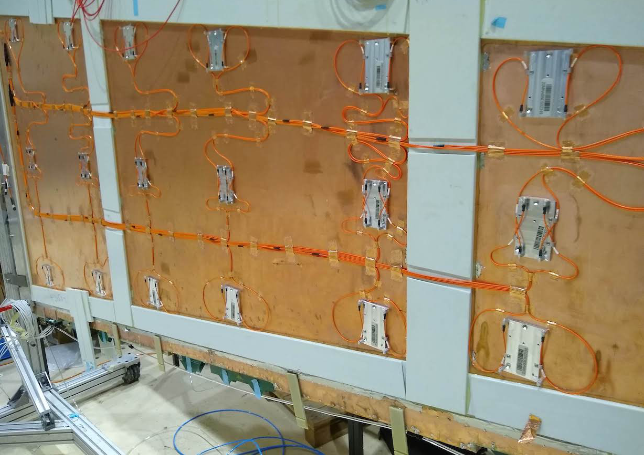
\includegraphics[width = 0.75\textwidth]{figures/alignment_platforms_lefebvre.png}
    \caption{A sTGC wedge with alignment platforms (silver) installed on the quadruplet. Optical fibres (orange) are routed to the alignment platforms. Cameras on the frames of the NSWs will record light from the optical fibres to monitor in real-time the position the alignment platforms in the ATLAS coordinate system.}
    \label{fig:alignment_platforms}
\end{figure}

% If you want to mention the alignment jig in the last paragraph:
% They are positioned with the help of an alignment jig, which is like a frame that can be positioned on top of a wedge with cut outs indicating the correct position for the alignment platforms. The jig is positioned with respect to the brass inserts \textcolor{red}{[Benoit 2020-01-20, 2020-04-16 presentations]}.

% The goal was to control the position of the strips in the chamber to within ~\SI{40}{\micro\meter} for precision tracking goals~\cite{nsw_tdr} --- then knowing the position of the brass inserts with respect to the alignment platforms would allow the strips to be positioned accurately enough. That is the alignment scheme shown in solid arrows in figure~\ref{fig:alignment_elements}. Due to time constraints, tolerances on the non-conformities in the etched strip pattern were loosened, with the condition that the strips positions would have to be corrected for in the software~\cite{carlson_results_2019}. Then, non-conformities in the brass inserts, misalignment of the pins the brass inserts were pushed against, and shifts of the strip layers while the glue was curing resulted in misalignments between the brass inserts~-- and between the strips layers ~-- that prevent using the brasses as an external reference of the position of the strips. The misalignments between Canadian sTGCs were shown to be random~\cite{carlson_results_2019}, so no one correction would suffice.

% The original alignment scheme was to use the brass inserts as a reference between the alignment platforms and the individual strips, as shown in the solid arrows in figure~\ref{fig:alignment_elements}. \textcolor{red}{Due to time constraints, tolerances on the non-conformities in the etched strip pattern with respect to the brass inserts were loosened, with the condition that the strips positions would have to be corrected for. Corrections will happen in ATLAS offline software, \package{Athena}, that will do the precision tracking~\cite{carlson_results_2019}. --> MOVE THIS} Moreover, non-conformities in the shape of the brass inserts and the alignment pins added misalignment between the inserts of different layers~-- and between the strips of different layers~-- that prevent using the brass inserts as a reference. Offsets in strip positions from nominal in Canadian quadruplets were shown to be random~\cite{carlson_results_2019}, so no one correction would suffice.

\begin{figure}
    \centering
    
\includegraphics[width = 0.9\textwidth]{figures/alignment_system_element_relations.png}
    \caption{Schematic diagram showing how the different elements of the sTGC alignment system relate to one another. The solid arrows denote the planned alignment scheme. The dashed arrow shows the modification being finalized now. This figure was originally designed by Dr. Benoit Lefebvre.}
    \label{fig:alignment_elements}
\end{figure}

The original alignment scheme was to use the brass inserts as a reference between the alignment platforms and the individual strips, as shown in the solid arrows in Figure~\ref{fig:alignment_elements}~-- this will no longer work. The position of the alignment platforms will be known thanks to the alignment system, so a different method to get the position of the strips with respect to the alignment platforms is currently in its final stage of development. The technique consists of the measurement of the strip pattern offset at a few areas on the surface of a sTGC quadruplet using an xray gun mounted on the alignment platforms. The local strip pattern offset with respect to nominal geometry at the location of each alignment platform is obtained by analyzing the xray gun beam profile. As shown in Figure~\ref{fig:alignment_elements}, this approach essentially bypasses the need to know the position of strips with respect to the brass inserts. The alignment platforms provide the link to the nominal geometry because the nominal group of strips that should be nearest to them can be identified using the nominal geometry parameters that assume the strips are perfectly etched and aligned. Cosmic muon track positions cannot be compared to the nominal geometry because the alignment platforms are not installed when cosmics data is collected, so there is no external reference to provide a link to the nominal geometry.

The x-ray method does not have the sensitivity to measure the offset of each strip from nominal, but what can be measured instead is the offset of the strip pattern in a local area around the position of the gun. \textit{Local offsets} are used to build an alignment model for each strip layer. Formally defined, an alignment model is a set of parameters used to estimate the ``as-built'' position of a strip given its nominal position. The alignment model currently being worked on takes x-ray and CMM data as input to calculate an overall offset and rotation of each strip layer with respect to nominal~\cite{lefebvre_precision_2020}. The alignment parameters could be described as ``global'', meaning over the whole layer instead of local. Without the x-ray dataset, there would be no input to the alignment model that takes into account inter-layer misalignments introduced during quadruplet construction.

Given that the x-ray local offsets can only be measured at positions where the gun can be attached and that they are an important part of the alignment scheme, the new x-ray measurement technique needs to be validated. The goal of this thesis is to validate the x-ray local offsets while exploring how cosmics data complements and adds to the understanding of strip positions and global alignment.

% --------------------------------------------------
% \section{Thesis motivation}
% --------------------------------------------------
%\textcolor{red}{It feels right to remind people of the goal of this work here, even though this is done in the introduction. Options: keep this section, remove this section; move the first two sentences of this section to the end of the NSW alignment section above for a briefer reminder. Thoughts?}

% Given that the x-ray local offsets can only be measured at positions where the gun can be attached and that they are an important part of the alignment scheme, the x-ray method needs to be validated. The goal of this thesis is to validate the x-ray local offsets while exploring how cosmics data complements and adds to the understanding of strip positions and overall alignment. Chapter~\ref{chap:lhc_atlas} presented the physics motivation of the HL-LHC and chapter~\ref{chap:nsw} motivated the NSW upgrade and the importance of alignment. Chapter~\ref{chap:cosmics} explains how cosmic muon data is collected, how it is used to calculate relative local offsets, and what information it gives about alignment. Chapter~\ref{chap:xray} explains how x-ray data is collected, how it is used to calculate local offsets, and how relative local offsets can be calculated for comparison to cosmics. Chapter~\ref{chap:comparison} compares the results of the two methods; and chapter~\ref{chap:outlook} contextualizes the results in terms of the alignment model and alignment system.

% Snippets
%The main dataset was collected using x-rays as the probe. The x-ray data has been combined with the CMM data to create an alignment model that can be used to estimate the position of each strip. The goal of this work was to validate the measurements of strip pattern offsets done with the x-ray dataset with the cosmic muon data. Currently, only modules made in Canada have been analyzed in this way, but the method applies for other countries that were able to collect cosmic muon data on multiple quadruplet layers. 

%Moreover, as-built alignment parameters must be measured and extracted to ensure proper function and provide a way to correct for misalignment. The next section breaks down the sTGC construction process to highlight the stages of alignment.
%All countries successfully finished delivering their modules this year, and the sectors have been installed on the NSWs. 






























